
\chapter{Introduction}\label{ch:introduction}

\begin{quotation}{\slshape
		An intelligent being cannot treat every object it sees as unique entity unlike anything else in the universe. It has to put objects in categories so that it may apply its hard-won knowledge about similar objects encountered in the past, to he object at hand.}
		\begin{flushright}
			\textbf{Steven Pinker, How the Mind Works, 1997} 
		\end{flushright}
\end{quotation}

One of the most basic and primitive abilities that human beings are endowed with is being able to group similar objects to produce a classification that is useful to them. For example, they should have been able to realize which objects were edible, which were poisonous, and which would try to kill them.

Classification skills, in their broadest sense, are necessary for language development, which is made up of words that help us recognize different types of events, actions and entities. In essence, each noun is a label that we use to group a collective of beings or objects with similar features, so that we can refer to them all using the word that unites them.

Just as classification is a basic skill for people in their daily lives, it is also essential in most branches of science. In biology, for example, the classification of different types of organisms has been the subject of study since the beginning of its existence. Aristotle built an elaborated animal classification system, dividing all creatures into two groups: red-blooded and not red-blooded. Later he proposed a subdivision that classified them according to the way in which new individuals came into the world, either alive, by means of eggs, chrysalis, etc.

Following Aristotle, Theophrastus wrote the first document compiling guidelines for the classification of plants. The resulting works were so extensive and detailed that they laid the foundation for research in biology over the following centuries. This work was not replaced until 1737, when Carl von Linné published his work \textit{Genera Plantarum}, from which we extract the following fragment:

\begin{quotation}{\slshape
		All the real knowledge which we possess, depends on methods by which we distinguish the similar from the dissimilar. The greater the number of natural distinctions this method comprehends the clearer becomes our idea of things. The
		more numerous the objects which employ our attention the more difficult it becomes to
		form such a method and the more necessary.
		For we must not join in the same genus the horse and the swine, though both species
		had been one hoof’d nor separate in different genera the goat, the reindeer and the elk,
		tho’ they differ in the form of their horns. We ought therefore by attentive and diligent
		observation to determine the limits of the genera, since they cannot be determined a
		priori. This is the great work, the important labour, for should the genera be confused,
		all would be confusion.} 
		\begin{flushright}
			\textbf{Carl von Linné, Genera Plantarum, 1737}
		\end{flushright}
\end{quotation}

Classification of animals and plants has been of major importance in fields such as biology and zoology. In particular, this classification laid the foundation for the development of Darwin's theory of evolution. But it has also been of high relevance in knowledge areas such as chemistry and physics, with the classification of the elements in the periodic table, proposed by Mendeleyev in the 1860s; or in astronomy, with the classification of dwarf or giant stars using the Hertzsprung-Russell guidelines, shown in Figure \ref{fig:intro_HRdiagram}.

\begin{figure}[!h]
	\centering
	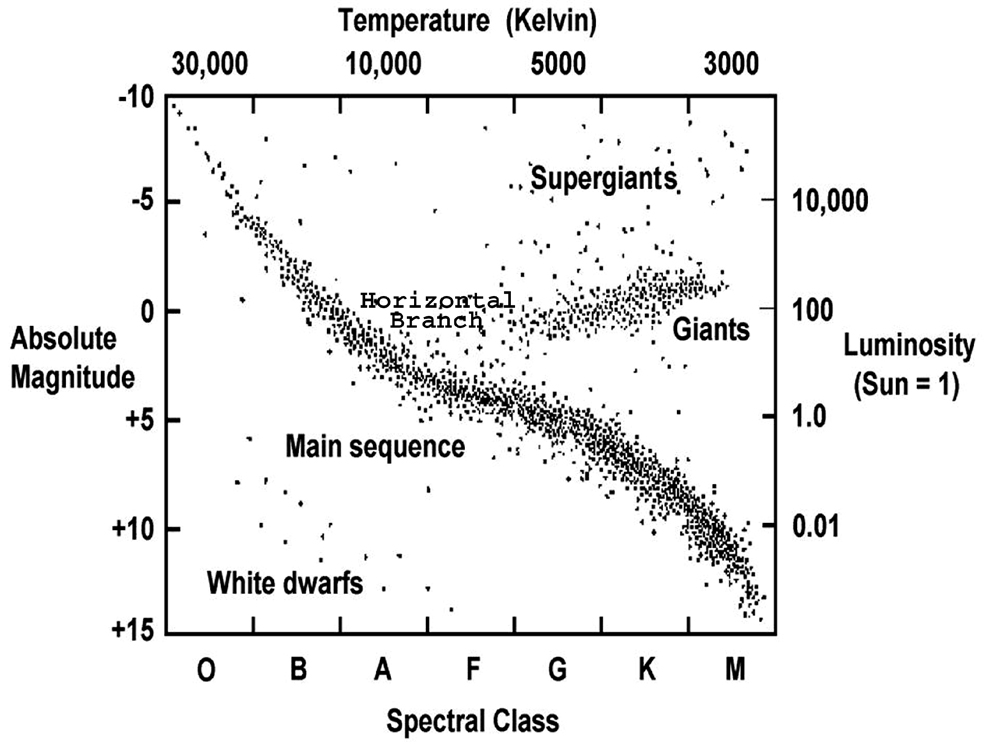
\includegraphics[scale=0.35]{gfx/Intro/HR_diagram} 
	\caption[Hertzsprung-Russell stars classification diagram.]{Hertzsprung-Russell stars classification diagram.}\label{fig:intro_HRdiagram}
\end{figure}

\section{The Learning Task}

We humans, like many other beings, are capable of learning a multitude of concepts throughout our lives, although generally the learning process is extremely slow. It takes us about six years to be able to begin dedicated and specific learning in primary education, and another eighteen years---generally speaking---to become computer scientists or experts in any other branch of knowledge.

Thus, the human learning process is a slow and tedious process. So, do we want to teach machines to learn the way humans do? Machines have proven to be outstanding at repetitive tasks, as well as they reach calculation speeds that humans can only dream of. It is worth asking if it is possible to develop a learning method for machines that is orders of magnitude faster than the human and equal or more effective. Although there is a major impediment to the development of such a method: we do not know if it exists! The search for a method to avoid the disadvantages of the human learning process is what drives research in the science we know today as \textit{machine learning}. 

One of the major differences between human learning and machine learning, and we must admit that to this respect machines again lead us, is the way in which knowledge is transferred. In machines it is enough to copy and paste, that is to say, once a program performs correctly the task for which it has been designed in a computer, it performs it in all of them. Just copy and paste. In humans this is not the case, we cannot extract knowledge from one brain and insert it into another, we don't even know how it is encoded! We humans must use our inefficient input-output devices to transmit knowledge. The following quote, which well reflects the reality of automatic learning, is more than thirty years old, yet still valid:

\begin{quotation}{\slshape
		...we do have reason to search for machine learning programs that will avoid the inefficiencies of human learning, although we must be alert to the possibility that such programs cannot, in principle, be constructed. The difficulty may be intrinsic in the task; human learning, though slow, may be close to optimally efficient.}
	\begin{flushright}
		\textbf{Herbert A. Simon, Machine Learning: An Artificial Intelligence Approach, 1983} 
	\end{flushright}
\end{quotation}

\section{Machine Learning}

So far, references have been made to learning without formally defining it. The concept of learning is deeply anchored in human beings. However, when trying to apply learning to computers, which are still no more than glorified calculators, we must give some kind of definition: \textit{Learning denotes changes in the system that are adaptive in the sense that they enable the system to do the same task or tasks drawn from the same population more efficiently and more effectively the next time} \cite{Michalski:2013:MLA:2588013}.

Machine learning is a field derived from computer science, and a branch of \acf{AI}, whose ultimate goal is to develop methods that make it possible for machines to learn. In other words, the techniques embedded in machine learning aim to develop programs that guide computers to learn from a set of examples. Machine learning is part of \acs{AI} in the sense that \acs{AI} is often directed at simulating human beings behavior through computers, so that we can better understand how humans work and help them.

\subsection{Types of Machine Learning} \label{sec:TypesOfML}

There are several approaches within the field of machine learning, these are classified according to the information that is provided to the machine for it to learn. Thus, following the classification proposed in \cite{ayodele2010types}, we find four different types of learning:

\begin{itemize}
	
	\item \textbf{Supervised Learning}: complete information is provided for learning. The machine is provided with a set of examples and the class (label) associated with each of them. The goal is to generate a function that approximates the behavior of the function that maps the examples in their respective classes.
	
	\item \textbf{Unsupervised Learning}: in this case the class to which the examples belong to is not available. The goal is to extract the class from the information contained in the set of examples.
	
	\item \textbf{Semi-supervised Learning}: it arises from adding incomplete information to unsupervised learning. This information is usually given in the form of a subset of labeled data, but there is no restrictions to this concern.
	
	\item \textbf{Reinforcement Learning}: the algorithm learns how to act under the influence of its environment, which provides feedback on the actions taken by the algorithm.
	
\end{itemize}

Among the four main categories of machine learning methods we find the \acf{SSL}, which is the focus of this work. As we have already mentioned, it is a machine learning paradigm that arises from adding incomplete information to unsupervised learning. We can divide \acs{SSL} methods into two broad categories according to their objective: semi-supervised classification and semi-supervised clustering \cite{chapelle2009semi}. The first method has partial information about the labels, so it tries to minimize the error based on them while taking into account the distribution of unlabeled instances. The second tries to obtain better defined clusters incorporating background information to the clustering process, this is known as constrained clustering and is the main subject of the study presented in this work \cite{triguero2015self}.

\section{Structure}
































